\section{Experiments}\label{sec:experiments}
Experiments are conducted in this section in order to answer the following research questions:
\begin{itemize}
    \item \textbf{RQ1}: How do the CSGCN models compare to state-of-the-art methods for the task of context-aware list prediction?
    \item \textbf{RQ2}: Can the CSGCN models be used to make non-context specific recommendations?
    \item \textbf{RQ3}: Does side-information improve results for context-aware recommendations?
\end{itemize}
The section details the experimental settings used, the datasets, the methods, and the metrics employed for comparison.

\subsection{Datasets}\label{subsec:experimental-settings}
To test the models on datasets with varying sizes and density, the following datasets were chosen:\\

\begin{adjustwidth}{-2.5 cm}{-2.5 cm}\centering
\begin{threeparttable}[]
\scriptsize
\begin{tabular}{lcccccc}\toprule
\textbf{Dataset} &\textbf{User \#} &\textbf{Item \#} &\textbf{Interaction \#} &\textbf{Context \#} &\textbf{Sideinfo \#} \\\cmidrule{1-6}
ML1m &6,040 &3,377 &999,416 &2 &4 \\\cmidrule{1-6}
%ML100k &943 &1,682 &100,000 &4 &4 \\\cmidrule{1-6}
Frappe &546 & 821 &85,541 &6 &1 \\\cmidrule{1-6}
Yelp-NC &2,274 &2,140 &130,627 &1 &3 \\\cmidrule{1-6}
Yelp-ON &5,185 &5,566 &332,291 &1 &3 \\\midrule
\bottomrule
\end{tabular}
\caption{Statistics of the datasets.}\label{tab:datasetstats}
\end{threeparttable}
\end{adjustwidth}

\subsubsection*{MovieLens 1M (ML1M)}
ML1M is a dataset \cite{ml1m} with 1 million interactions between 6,040 users and 3,377 movies.\\
We use the following side-information for users:
\begin{itemize}
    \item Age
    \item Gender
    \item Occupation
\end{itemize}
Side-information for items is \textit{genre}, which specifies that an item has one or more of the 18 genres available in the dataset.
For contextual information, the MovieLens dataset provides a timestamp for when the interaction took place.

\subsubsection*{Frappe}
The Frappe dataset \cite{baltrunasfrappe} contains information about how users have interacted with applications on their smartphones.
The only available side-information is for items, indicating whether the application is free or not.
However, it contains the following contexts:
\begin{itemize}
    \item City
    \item Country
    \item Weekday
    \item Time of day
    \item Whether it is weekend or not
    \item Weather
\end{itemize}

\subsubsection*{Yelp-NC and Yelp-ON}
The two Yelp datasets, Yelp-NC and Yelp-ON, are subsets of the public Yelp dataset \cite{yelp}, where we take the subset of items located in respectively North Carolina (NC) and Ontario (ON).
Both Yelp datasets have been pruned such that it includes only users with at least 10 interactions, to facilitate generating a stratified data split where each user in the test set is also in the training set.\\
We use the following side-information about users for both datasets:
\begin{itemize}
    \item Yelping since (Year)
    \item Number of fans
    \item Average stars
\end{itemize}
The side-information about items is a dimension specifying the categories that an item belongs to.
For the Yelp-NC dataset, this is one or more of 80 different categories, and 75 categories for Yelp-ON.\\
The contextual information is a timestamp.

\subsection{Context dimension selection}
Since most of the datasets include a timestamp as contextual information, we discretize these into the following context dimensions:
\begin{itemize}
    \item Month
    \item Day of week
    \item Hour
    \item Time of day
\end{itemize}
Where time of day is a further discretization of the hour dimension, split into 5 intervals:
\begin{itemize}
    \item Night (0 to 4)
    \item Early morning (4 to 8)
    \item Late morning (8 to 12)
    \item Evening (12 to 16)
    \item Afternoon (16 to 20)
    \item Late night (20 to 24)
\end{itemize}
For the Frappe dataset, we instead make use of the 6 contextual values available in the dataset.
\\\\
For the side-information, we use the dimensions mentioned in \Cref{subsec:experimental-settings} for both users and items with some discretization.
The Yelp datasets provide a "yelping since" dimension, which is a timestamp for the creation of the user.
This is discretized to include only the year that the user has been created.
\\
Additionally, the dimension "fans" is discretized into four groups:
\begin{itemize}
    \item $< 50$ fans
    \item $50 - 100$ fans
    \item $100-500$ fans
    \item $> 500$ fans
\end{itemize}

\subsection{Compared methods}
In the experiments, the CSGCN models are compared against the following methods for context-specific recommendations:
\begin{itemize}
    \item Factorization Machine (FM) \cite{fmrendle}
    \item Convolutional Factorization Machine (CFM) \cite{CFM}
    \item Neural Factorization Machine (NFM) \cite{NeuralFM}
    % \item Top Pop
    % \item CAMF \cite{CAMF}
\end{itemize}
FM is a relatively simple model that models all interactions between variables using factorized parameters.
It is often used for comparison in context-aware papers, since it is able to predict a score based on information about a given interaction including contextual information.
CFM uses a combination of a CNN and an FM, which is similar to our method in that it is capable of producing a context-aware top-$k$ recommendation list.
It is included since it is an alternative way to handle contextual information in CNNs.
We also compare against NFM, which uses a multi-layer perceptron (MLP) on top of the factorization machine to learn higher-order interaction signals.
\\\\
To compare the performance of the models in a non-context specific setting, we compare against the following methods:
\begin{itemize}
    \item Neural Graph Collaborative Filtering (NGCF) \cite{NGCF}
    \item Light Graph Convolutional Network (LightGCN) \cite{LightGCN}
    \item Knowledge Graph Attention Network (KGAT) \cite{KGAT}
    \item Bayesian Personalized Ranking (BPR) \cite{BPR}
    \item Top Pop
    %\item Factorization Machine \cite{fmrendle}
\end{itemize}
NGCF is a model proposed by Wang et al. as a way to utilize the GCN model proposed in \cite{KOrderConnectivity} for recommendation purposes.
It makes use of all three parts of a GCN described in \Cref{sec:preliminaries}, and utilizes BPR loss with negative sampling to use it for a ranking purpose.
LightGCN was later proposed by the same authors and is mainly focused on performing an ablation study similar to the one done in \cite{SimplifyingGCN}, where they remove the linear transformation and non-linear activation between layers to provide a simpler model, while still presenting competitive results.
Both the CSGCN models and LightGCN extend the codebase of NGCF, so they are naturally included in the comparison to show that adding side-information and contextual information hopefully improves the accuracy of these methods.\\
KGAT is a state-of-the-art graph-based method that utilizes side-info in the form of a knowledge graph.
BPR utilizes implicit feedback to generate a personalized top-$k$ list of items using the proposed BPR-optimizer to train the model, providing a simpler method for comparison.
Finally, a we include a simple baseline, Top Pop, which simply recommends the $k$ most popular items for all users.

\subsection{Parameter settings}
To fairly compare the performance of the models, we train all of them by optimizing the BPR loss with Adam.
The learning rate is either set to the value presented in the respective papers, or searched between $[0.1, 0.01, 0.001, 0.0001]$ if a default is not available.
The batch size is set as 1024 for all datasets except Frappe, where it is set to 512 due to its size.
The embedding size is set to 64, and for the models using regularization terms, this is searched between $[0.01, 0.001, 0.0001]$ if a default value is not provided.
For CFM and NFM we follow the approach presented in the original papers and feed them with weights from a pretrained FM model which has run for 500 epochs with the settings presented in the CFM paper.
All methods are run for a max of 1000 epochs with an early stopping mechanism triggered when the HR@20 or Recall@20 has not improved for 5 evaluations (100 consecutive steps), except for CFM which is run for 300 epochs based on the default values.


\subsection{Evaluating the models}\label{subsec:evalandmetrics}
The objectives of the models in the experiments are to produce top-$k$ lists of items for a user. 
Different methods for evaluating the performances of the models were considered, specifically the fold-out and leave-one-out methods.
These methods interact with the context in different ways.
For the fold-out method, the datasets are split into a training set and a test set, where the model is trained on the training set and evaluated on the test set. 
This split is generated such that each user in the test set is also found in the training set.
Using this stratified split method, we decided to use a split of 80\% training and 20\% test split.
Because of this split, a single user can have multiple ground truth entries across multiple contexts.\\
A problem to consider with fold-out for context-aware evaluation is that when the context is part of the input to the model, a score must be calculated for each combination of item and context due to the multiple ground truth contexts, which can be computationally expensive.
A single context cannot be guaranteed for the user for all ground truths, and thus every context needs to be evaluated.
\\\\
For the leave-one-out method, the newest interaction for each user is removed from the training set and used as the test set, as per \cite{CFM, BPR}.
This means that when a top-$k$ list is produced for a user, only a single item amongst the recommended items can be relevant, and thus there is only one context within which the ground truth had occurred.
This approach is largely inspired by sequential recommendation systems, where you leave out the newest interaction from each user and try to predict the next item in the sequence based on the sequence of the previous interactions by the user \cite{aggarwal2016recommender}.\\
This approach limits the number of different metrics that can be used for this type of evaluation method.
\\\\
For comparisons we conduct an experiment using fold-out for models that produce a top-$k$ recommendation list and conduct a separate leave-one-out evaluation for models that produce a context-aware top-$k$ recommendation list. 
The metrics used for the fold-out evaluation are Precision, Recall, and Normalized Discounted Cumulative Gain (NDCG), while the leave-one-out experiments report Hit Rate (HR) and Mean Reciprocal Rank (MRR).

\subsubsection*{Evaluation metrics explained}
The top-$k$ recommendation problem is the task of recommending a list $L(u)$ to an active user $u$ containing $k$ items.
Evaluating the quality of a method can be done by splitting the set of items $I$ into a training set $I_{train}$ and a test set $I_{test}$ for each user.
\\
Let $T(u)$ be the the set of items that the user has interacted with in the test set.
Precision can be calculated according to \Cref{eqn:precision}, and recall according to \Cref{eqn:recall}.
Precision defines the proportion of relevant items among the predicted items, while recall is the proportion of items that were correctly predicted according to the ground truth.
\begin{equation}
    \label{eqn:precision}
    Precision@N(L) = \frac{1}{|U|} \sum\limits_{u \in U}\frac{|L(u) \cap T(u)|}{|L(u)|}
\end{equation}
\begin{equation}
    \label{eqn:recall}
    Recall@N(L) = \frac{1}{|U|} \sum\limits_{u \in U} \frac{|L(u) \cap T(u)|}{|T(u)|}
\end{equation}
Another metric to be used is NDCG \cite{dcgpaper}.
Assuming each user $u$ has a gain $g_{ui}$ from being recommended item $i$, then the average DCG for a list of $J$ items is defined in \Cref{eqn:dcg}, where $i_j$ is the item at position $j$ in the list, and the logarithm base $b$ is $2$ to ensure all positions are discounted.
This metric rewards lists that frontload relevant items.
\begin{equation}
    \label{eqn:dcg}
    DCG@N = \frac{1}{|U|} \sum\limits_{u=1}^{|U|} \sum\limits_{j = 1}^{|J|} \frac{g_{ui_j}}{log_b (j+1)}
\end{equation}
NDCG is defined in \Cref{eqn:ndcg}, where $iDCG$ is the ideal DCG, which is defined by sorting the recommended items such that the relevant items appear at the start of the list, resulting in the largest possible DCG value.
\begin{equation}
    \label{eqn:ndcg}
    NDCG@N = \frac{DCG}{iDCG}
\end{equation}
MRR \cite{MRR} is employed for the leave-one-out evaluation, defined in \Cref{eqn:mrr}.
For each user $u$ in $U$, MRR is calculated by finding the rank $r_u$ of the first relevant recommendation for each list, and then taking the mean of these ranks.
\begin{equation}
    \label{eqn:mrr}
    MRR@N = \frac{1}{|U|} \sum\limits_{u \in U}\frac{1}{r_u}
\end{equation}
The final metric used is HR.
If a relevant item for a user appears in the top-$k$ list, the $HR(u)$ for that user is $1$, otherwise it is $0$.
The final HR score is then calculated by taking the mean of all users' individual HR scores, as seen in \Cref{eqn:hr}.
\begin{equation}
    \label{eqn:hr}
    HR@N = \frac{1}{|U|} \sum\limits_{u \in U}HR(u)
\end{equation}

\subsection{Performance Comparison with Context (RQ1)}\label{subsec:rq1}
For the first research question we want to examine how the CSGCN models compare to state-of-the-art methods within context-aware list prediction.
To investigate this, the leave-one-out method presented in \Cref{subsec:evalandmetrics} is used, such that a single interaction is left out for each user, and a list is produced based on the context that this interaction took place in.

\begin{table*}[]
\centering
\resizebox{\textwidth}{!}{%
\begin{tabular}{c|l|cccc|cc}
Dataset & Metric & FM & \multicolumn{1}{c}{NFM} & \multicolumn{1}{c}{CFM} & \multicolumn{1}{c|}{CSGCN-IS} & \multicolumn{1}{c}{CSGCN-ADJ} & \multicolumn{1}{c|}{Impr.} \\ \hline
\multirow{4}{*}{Yelp-NC} & HR@20  & 0.0075  & 0.0142  & 0.0070 & 0.0625 & 0.0761  &  \\
                        & HR@50  & 0.0198  & 0.0240  & 0.0163 & 0.1143 & 0.1464  &  \\
                        & MRR@20 & 0.0022  & 0.0030  & 0.0037 & 0.0127 & 0.0158  &  \\
                        & MRR@50 & 0.0025  & 0.0033  & 0.0040 & 0.0143 & 0.0179  &  \\ \hline
\multirow{4}{*}{Frappe} & HR@20  & 0.6590  & 0.3516  & 0.3242 & 0.0458 & 0.0604  &  \\
                        & HR@50  & 0.8004  & 0.4945  & 0.4560 & 0.1062 & 0.1245  &  \\
                        & MRR@20 & 0.2895  & 0.1117  & 0.1032 & 0.0128 & 0.0184  &  \\
                        & MRR@50 & 0.2942  & 0.1166  & 0.1074 & 0.0146 & 0.0204  &  \\ \hline
\multirow{4}{*}{Yelp-ON} & HR@20  & 0.0083  & 0.0085  & 0.0073 & 0.0399 & 0.0534  &  \\
                        & HR@50  & 0.0133  & 0.0152  & 0.0133 & 0.0714 & 0.0997  &  \\
                        & MRR@20 & 0.0019  & 0.0021  & 0.0019 & 0.0091 & 0.0123  &  \\
                        & MRR@50 & 0.0020  & 0.0023  & 0.0021 & 0.0101 & 0.0137  &  \\ \hline
\multirow{4}{*}{ML1M}   & HR@20  & 0.0874  & 0.0937  &        & 0.1402 & 0.1652  &  \\
                        & HR@50  & 0.1856  & 0.2005  &        & 0.2603 & 0.2982  &  \\
                        & MRR@20 & 0.0199  & 0.0209  &        & 0.0336 & 0.0372  &  \\
                        & MRR@50 & 0.0229  & 0.0242  &        & 0.0373 & 0.0413  & 
\end{tabular}%
}
\caption{Results for context-specific recommendations.}
\label{tab:context-specific-table}
\end{table*}
The results for this experiment can be seen on \Cref{tab:context-specific-table}.
It is easily seen that both CSGCN-IS and CSGCN-ADJ outperform the various factorization machines on most datasets.
The exception is Frappe, a dataset that is fairly unbalanced in terms of which items have been interacted with. 
The twenty most popular items have between 640 and 6,634 interactions, which is quite a large number for a dataset only containing 85,541 interactions, meaning that almost every 13th interaction will involve the most popular item, whereas all items have a mean of 104 interactions.\\\\
From this, we can assume that the CSGCN-IS and CSGCN-ADJ methods work best on fairly balanced datasets, whereas factorization machines seem to have an advantage on datasets with highly popular items.\\\\
Another interesting observation from the data is that even though CFM is run on pretrained FM data as described in their paper, it generally performs worse than the traditional FM.
Additionally, the runtime of CFM is significantly higher than any of the other methods.
Running 300 epochs on an NVIDIA DGX-2 cloud takes several days, while CSGCN-ADJ can perform the same amount of epochs in just a matter of hours.
Due to the sheer amount of time required to fine-tune the hyperparameters, CFM has been run only once with the settings presented in the original paper.\\
We are not able to fairly compare with the results presented in the CFM paper, since they perform a different split of the data to perform their leave-one-out evaluation.
According to their paper, they take the latest interaction of each user - but looking at the actual datasets they provide, their test datasets are significantly larger than the number of users, meaning that their evaluation must be different from ours.
\\
In conclusion, the performance of the CSGCN models depends on the dataset characteristics.
While the models perform significantly worse than simpler models on the Frappe dataset, we would argue that this dataset is not an accurate representation of a real world scenario.

\subsection{Performance Comparison without Context (RQ2)}
Since the CSGCN models use context to generate a top-$k$ list in each context for each user.
We argue that this context information can be useful even for non-context-specific settings.
Imagine that your system is recommending businesses to users, and you have a business that is only open on Christmas.
On Christmas night, millions upon millions of users interact with this item, but it is never interacted with in any other context.
In a regular RS this would be seen as a popular item, since a lot of users have interacted with it.
However, looking at the context, we are able to infer that it is only in this exact context it is popular.
This leads to the item having a high likelihood of being recommended in exactly one context, but a low likelihood in any other.
With this in mind, we will try to answer RQ2 about whether the models can be used to make non-context specific recommendations through aggregations by investigating various types of aggregations of the scores.
The simplest solution would be to take the highest score for an item, regardless of the context that it was recommended for.
However, this may prove problematic, since an item may score highly in a single context but very low in any other context, as in the example before.\\
Instead, we propose to take an average score across all contexts.
With this, the item that is only interacted with in exactly one context has its score lowered by a factor of the number of contexts observed.

% Please add the following required packages to your document preamble:
% \usepackage{booktabs}
% \usepackage{multirow}
% \usepackage{graphicx}
% \usepackage[normalem]{ulem}
% \useunder{\uline}{\ul}{}
\begin{table*}[]
\resizebox{\textwidth}{!}{%
\begin{tabular}{@{}l|l|cccccc|cc@{}}
\multicolumn{1}{l|}{Dataset} &
  Metric &
  \multicolumn{1}{l}{LightGCN} &
  \multicolumn{1}{l}{KGAT} &
  \multicolumn{1}{l}{BPR} &
  \multicolumn{1}{l}{NGCF} &
  \multicolumn{1}{l}{TopPop} &
  \multicolumn{1}{l|}{CSGCN-IS} &
  \multicolumn{1}{l}{CSGCN-ADJ} &
  \multicolumn{1}{l|}{Impr.} \\ \midrule
\multirow{8}{*}{Yelp-NC} & Recall@20    & {\ul{0.1069}} & 0.1064       & 0.0971          & 0.0923 & 0.0625          & 0.1115 & \textbf{0.1143} &  \\
                        & Recall@50    & {\ul{0.1959}} & 0.1935       & 0.1802          & 0.1748 & 0.1226          & 0.2020 & \textbf{0.2058} &  \\
                        & Precision@20 & {\ul{0.0540}} & 0.0513       & 0.0482          & 0.0458 & 0.0308          & 0.0547 & \textbf{0.0575} &  \\
                        & Precision@50 & {\ul{0.0402}} & 0.0388       & 0.0362          & 0.0355 & 0.0247          & 0.0410 & \textbf{0.0425} &  \\
                        & NDCG@20      & {\ul{0.0953}} & 0.0843       & 0.0765          & 0.0786 & 0.0489          & 0.0995 & \textbf{0.1020} &  \\
                        & NDCG@50      & {\ul{0.1265}} & 0.0994       & 0.0907          & 0.1079 & 0.0588          & 0.1315 & \textbf{0.1341} &  \\
                        & F1@20        & {\ul{0.0717}} & 0.0692       & 0.0644          & 0.0612 & 0.0413          & 0.0734 & \textbf{0.0765} &  \\
                        & F1@50        & {\ul{0.0666}} & 0.0646       & 0.0603          & 0.0589 & 0.0411          & 0.0682 & \textbf{0.0704} &  \\ \midrule
\multirow{8}{*}{Frappe} & Recall@20    & 0.1101       & 0.1279       & {\ul{0.1404}}    & 0.1029 & \textbf{0.3787} & 0.1054 & 0.1129          &  \\
                        & Recall@50    & 0.1414       & 0.1700       & {\ul{0.1762}}    & 0.1340 & \textbf{0.5175} & 0.1376 & 0.1417          &  \\
                        & Precision@20 & 0.0553       & 0.0495       & {\ul{0.0591}}    & 0.0501 & \textbf{0.1687} & 0.0506 & 0.0576          &  \\
                        & Precision@50 & 0.0306       & 0.0289       & {\ul{0.0311}}    & 0.0284 & \textbf{0.0968} & 0.0291 & 0.0304          &  \\
                        & NDCG@20      & 0.1141       & 0.0978       & {\ul {0.1340}}    & 0.0986 & \textbf{0.3695} & 0.0997 & 0.1207          &  \\
                        & NDCG@50      & 0.1203       & 0.1085       & {\ul {0.1377}}    & 0.1057 & \textbf{0.3775} & 0.1073 & 0.1245          &  \\
                        & F1@20        & 0.0736       & 0.0714       & {\ul {0.0832}}    & 0.0674 & \textbf{0.2335} & 0.0671 & 0.0763          &  \\
                        & F1@50        & 0.0503       & 0.0495       & {\ul {0.0529}}    & 0.0468 & \textbf{0.1632} & 0.0480 & 0.0501          &  \\ \midrule
\multirow{8}{*}{Yelp-ON} & Recall@20    & {\ul {0.0748}} & 0.0700       & 0.0658          & 0.0603 & 0.0360          & 0.0751 & \textbf{0.0809} &  \\
                        & Recall@50    & {\ul {0.1354}} & 0.1321       & 0.1227          & 0.1157 & 0.0681          & 0.1378 & \textbf{0.1477} &  \\
                        & Precision@20 & {\ul {0.0425}} & 0.0395       & 0.0380          & 0.0342 & 0.0200          & 0.0432 & \textbf{0.0456} &  \\
                        & Precision@50 & {\ul {0.0311}} & 0.0297       & 0.0285          & 0.0267 & 0.0156          & 0.0316 & \textbf{0.0335} &  \\
                        & NDCG@20      & {\ul {0.0699}} & 0.0610       & 0.0570          & 0.0554 & 0.0303          & 0.0713 & \textbf{0.0769} &  \\
                        & NDCG@50      & {\ul {0.0909}} & 0.0703       & 0.0656          & 0.0755 & 0.0356          & 0.0928 & \textbf{0.1000} &  \\
                        & F1@20        & {\ul {0.0542}} & 0.0505       & 0.0481          & 0.0436 & 0.0258          & 0.0549 & \textbf{0.0583} &  \\
                        & F1@50        & {\ul {0.0506}} & 0.0485       & 0.0463          & 0.0433 & 0.0255          & 0.0514 & \textbf{0.0547} &  \\ \midrule
\multirow{8}{*}{ML1M}   & Recall@20    & 0.2481       & 0.2465       & {\ul {0.2642}}    & 0.2291 & 0.0827          & 0.2550 & \textbf{0.2675} &  \\
                        & Recall@50    & 0.4144       & 0.4125       & {\ul {0.4330}}    & 0.3874 & 0.1633          & 0.4185 & \textbf{0.4351} &  \\
                        & Precision@20 & 0.2885       & 0.2874       & \textbf{0.3015} & 0.2663 & 0.0864          & 0.2923 & {\ul {0.3013}}    &  \\
                        & Precision@50 & 0.2110       & 0.2099       & \textbf{0.2189} & 0.1965 & 0.0734          & 0.2125 & {\ul {0.2180}}    &  \\
                        & NDCG@20      & 0.3754       & {\ul{ 0.3971}} & \textbf{0.4184} & 0.3443 & 0.1044          & 0.3822 & {\ul {0.3971}}    &  \\
                        & NDCG@50      & 0.3966       & 0.3874       & {\ul {0.4087}}    & 0.3662 & 0.1144          & 0.4027 & \textbf{0.4178} &  \\
                        & F1@20        & 0.2668       & 0.2654       & {\ul{0.2816}}    & 0.2463 & 0.0845          & 0.2724 & \textbf{0.2834} &  \\
                        & F1@50        & 0.2797       & 0.2782       & \textbf{0.2907} & 0.2608 & 0.1013          & 0.2819 & {\ul{0.2905}}    &  \\ \bottomrule
\end{tabular}%
}
\caption{Results for the aggregated results.}
\label{tab:aggregatedresults}
\end{table*}
The results for the non-context-specific recommendation task can be seen in \Cref{tab:aggregatedresults}.
Generally, we see that both CSGCN methods are among the best performers across all metrics on the datasets, with CSGCN-ADJ outperforming CSGCN-IS on all metrics.
The main exception is on the Frappe dataset, where BPR and KGAT perform significantly better.
We suspect that this is due to the density and small size of the dataset.
Frappe has a density of 18.9\%, compared to the others that range between 1.1\% and 4.8\%, allowing for simpler methods like BPR to perform better relative to other datasets, whereas complex methods like NGCF struggle to learn properly.
Even more interesting in the Frappe dataset is the performance of TopPop, which outperforms all other methods on all metrics.
This is most likely caused by the dataset including some very popular items as described in \Cref{subsec:rq1}.
All of these results are based on using the mean aggregator, but for the sake of completeness, let us compare the performance for the Yelp-ON dataset across various aggregators of context on CSGCN-IS.

\begin{figure}
    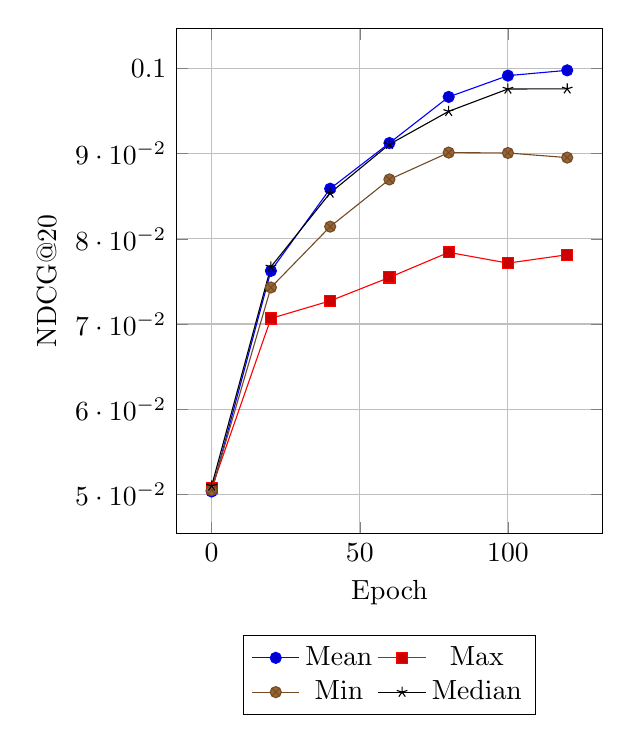
\begin{tikzpicture}
        \begin{axis}[
            xlabel=Epoch,
            ylabel=NDCG@20,
            height=8cm,
            width=7cm,
            grid=major,
            legend style={at={(0.5,-0.20)},
        anchor=north,legend columns=2}]
            
        \addplot plot coordinates{
            (0,0.05035)
            (20,0.07624)
            (40,0.08588)
            (60,0.09124)
            (80,0.09665)
            (100,0.09915)
            (120,0.09977)
        };

        \addplot plot coordinates{
            (0,0.05072)
            (20,0.07066)
            (40,0.07272)
            (60,0.07547)
            (80,0.07841)
            (100,0.07715)
            (120,0.07813)
        };

        \addplot plot coordinates{
            (0,0.05051)
            (20,0.07429)
            (40,0.08143)
            (60,0.08697)
            (80,0.09012)
            (100,0.09007)
            (120,0.08953)
        };
        
        \addplot plot coordinates{
            (0,0.051)
            (20,0.07671)
            (40,0.08538)
            (60,0.09109)
            (80,0.09496)
            (100,0.09758)
            (120,0.0976)
        };

        \legend{Mean,Max,Min,Median}
        \end{axis}
    \end{tikzpicture}
    \caption{Effect of aggregation functions for CSGCN-IS on the Yelp-NC dataset for NDCG@20.}
    \label{fig:aggregation_effect}
\end{figure}
\Cref{fig:aggregation_effect} shows how the choice of aggregation affects the CSGCN-IS model.
This shows that using a mean aggregation function provides the best results, followed by the median.
The simple solution of taking the lowest or highest score across the contexts is shown at the bottom of the graph.\\
This supports the previous assumption that while a single item might be more likely to be recommended in one context, it does not necessarily mean that it is a good recommendation overall, which is better captured through the mean or median aggregations.\\
While the results are only shown for NDCG@20 for this dataset, they have proven consistent across all the metrics.

\subsubsection*{Ablation study for non-contextual recommendation}
To test whether context and side-information actually increase performance in a non-context specific setting, CSGCN-ADJ is run using different inputs for the datasets Yelp-NC and ML1M and the performance is measured with NDCG@20.
First of all, CSGCN-ADJ is run with both side-information and context. 
Then side-information is removed, followed by removing context, and finally both context and side-information are removed.
\begin{figure*}[t!]
    \captionsetup{justification=centering}
    \begin{subfigure}[t]{0.4\textwidth}
        \captionsetup{justification=centering,margin={0cm,2.1cm}}
        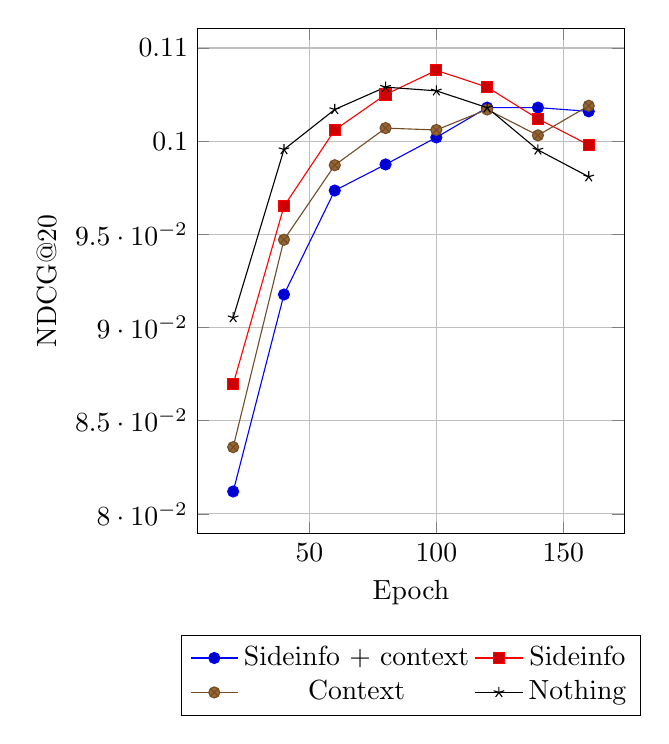
\begin{tikzpicture}
            \begin{axis}[
                xlabel=Epoch,
                ylabel=NDCG@20,
                height=8cm,
                width=7cm,
                grid=major,
                legend style={at={(0.5,-0.20)},
            anchor=north,legend columns=2}]
                
            \addplot plot coordinates{
                (20,8.120e-02)
                (40,9.177e-02)
                (60,9.735e-02)
                (80,9.875e-02)
                (100,1.002e-01)
                (120,1.018e-01)
                (140,1.018e-01)
                (160,1.016e-01)
            };
    
            \addplot plot coordinates {
                (20,8.696e-02)
                (40,9.651e-02)
                (60,1.006e-01)
                (80,1.025e-01)
                (100,1.038e-01)
                (120,1.029e-01)
                (140,1.012e-01)
                (160,9.98e-02)
            };
    
            \addplot plot coordinates {
                (20,8.358e-02)
                (40,9.471e-02)
                (60,9.871e-02)
                (80,1.007e-01)
                (100,1.006e-01)
                (120,1.017e-01)
                (140,1.0031e-01)
                (160,1.019e-01)
            };
    
            \addplot plot coordinates {
                (20,9.053e-02)
                (40,9.955e-02)
                (60,1.017e-01)
                (80,1.029e-01)
                (100,1.027e-01)
                (120,1.018e-01)
                (140,9.953e-02)
                (160,9.809e-02)
    
            };
            \legend{Sideinfo + context,Sideinfo,Context,Nothing}
            \end{axis}
        \end{tikzpicture}
        \caption{The performance on NDCG@20 of CSGCN-ADJ on the Yelp-NC dataset with different types of input.}
        \label{fig:ablation_study_non_context_1}
    \end{subfigure}
    \hspace{0.1\textwidth}
    \begin{subfigure}[t]{0.4\textwidth}
        \captionsetup{justification=centering,margin={0cm,1cm}}
        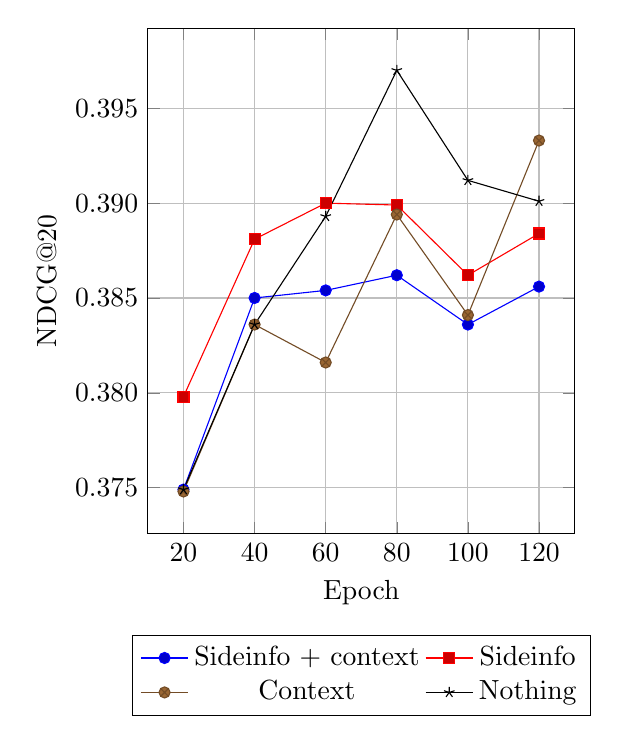
\begin{tikzpicture}
            \begin{axis}[
                ytick={0.370,0.375,0.380,0.385,0.390,0.395,0.40},
                xlabel=Epoch,
                ylabel=NDCG@20,
                height=8cm,
                width=7cm,
                y tick label style={
                    /pgf/number format/.cd,
                    fixed,
                    fixed zerofill,
                    precision=3,
                    /tikz/.cd
                },
                grid=major,
                legend style={at={(0.5,-0.20)},
            anchor=north,legend columns=2}]
                
            \addplot plot coordinates{
                (20,0.3749)
                (40,0.3850)
                (60,0.3854)
                (80,0.3862)
                (100,0.3836)
                (120,0.3856)
            };
    
            \addplot plot coordinates {
                (20,0.3798)
                (40,0.3881)
                (60,0.3900)
                (80,0.3899)
                (100,0.3862)
                (120,0.3884)
            };
    
            \addplot plot coordinates {
                (20,0.3748)
                (40,0.3836)
                (60,0.3816)
                (80,0.3894)
                (100,0.3841)
                (120,0.3933)
            };
    
            \addplot plot coordinates {
                (20,0.3749)
                (40,0.3836)
                (60,0.3893)
                (80,0.3970)
                (100,0.3912)
                (120,0.3901)
            };
            \legend{Sideinfo + context,Sideinfo,Context,Nothing}
            \end{axis}
        \end{tikzpicture}
        \caption{The performance on NDCG@20 of CSGCN-ADJ on the ML1M dataset with different types of input.}
        \label{fig:ablation_study_non_context_2}
    \end{subfigure}
    \caption{Ablation study for the input of CSGCN-ADJ on Yelp-NC and ML1M.}
    \label{fig:inputablation}
\end{figure*}
\Cref{fig:ablation_study_non_context_1} shows the performance on NDCG@20 of CSGCN-ADJ with different input.
It shows that the more input the model receives, the longer it takes to converge to its best performance.
Overall, the performance does not change drastically with the different types of input.
Having only side-information as input achieves the best performance, but it is only marginally better than not having side-information and context at all.
Having both context and side-information actually degrades performance slightly, compared to just having side-information as the input, and having just context as input improves performance slightly.
To conclude from the study on the Yelp-NC dataset, the usage of context is not able to provide better recommendations in a non-context-specific setting.
Side-information, however, performs the best on this metric on this dataset, which suggests that side-information in CSGCN-ADJ is able to slightly improve results compared to having no extra input.
\\
On \Cref{fig:ablation_study_non_context_2} the NDGC@20 results of ML1M are shown for CSGCN-ADJ with different types of input. 
For this dataset, the model that uses neither the context nor side-information for the input is actually the best performing version.
Side-information and context are not able to improve the performance of CSGCN-ADJ on ML1M in a non-context-specific setting.
Since both \Cref{fig:ablation_study_non_context_1,fig:ablation_study_non_context_2} show that the model is worse with context included, it can be concluded that context does not increase the performance of CSGCN-ADJ in a non-context specific setting.
Side-information, however, is able to increase performance of the model in a non-context specific setting, but for this dataset the side-information does not provide any additional collaborative signal.

\subsection{Ablation study of model extensions (RQ3)}
To answer whether side-information improves the results for context-aware recommendations, we performed an ablation study on the Yelp-NC dataset.
In the study, the CSGCN models were run with and without side-information to test the effect it has on the performance.
Additionally, the experiment was conducted on the context input to examine how much it affects the performance in a context-specific setting.
\begin{figure*}[t!]
    \captionsetup{justification=centering}
    \begin{subfigure}[t]{0.4\textwidth}
        \captionsetup{justification=centering,margin={1.4cm,-1.3cm}}
        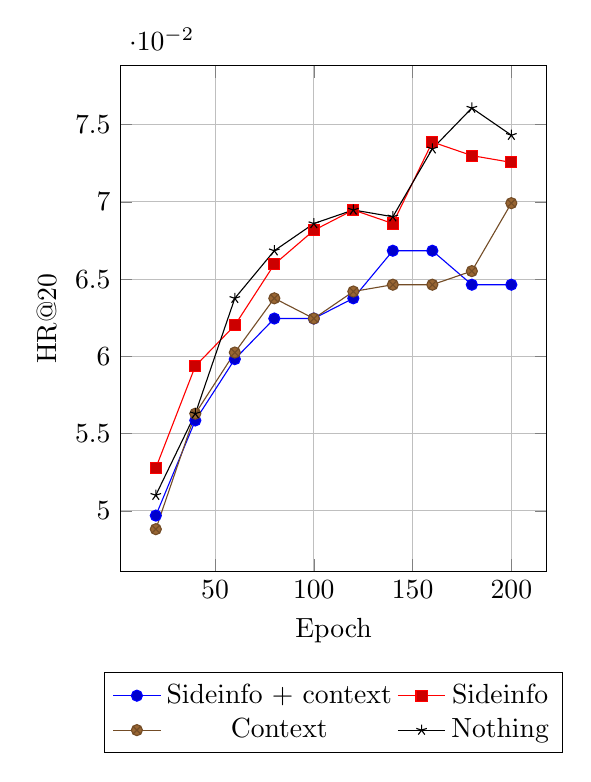
\begin{tikzpicture}
        \begin{axis}[
            xlabel=Epoch,
            ylabel=HR@20,
            height=8cm,
            width=7cm,
            grid=major,
            legend style={at={(0.5,-0.20)},
        anchor=north,legend columns=2}]
            
        \addplot plot coordinates{
            (20,0.04969)
            (40,0.05585)
            (60,0.05982)
            (80,0.06245)
            (100,0.06245)
            (120,0.06376)
            (140,0.06684)
            (160,0.06684)
            (180,0.06464)
            (200,0.06464)
        };

        \addplot plot coordinates {
            (20,0.05277)
            (40,0.05937)
            (60,0.06201)
            (80,0.06596)
            (100,0.06816)
            (120,0.06948)
            (140,0.06860)
            (160,0.07388)
            (180,0.07300)
            (200,0.07256)
        };

        \addplot plot coordinates {
            (20,0.04881)
            (40,0.05629)
            (60,0.06025)
            (80,0.06376)
            (100,0.06245)
            (120,0.06420)
            (140,0.06464)
            (160,0.06464)
            (180,0.06552)
            (200,0.06992)
        };

        \addplot plot coordinates {
            (20,0.05101)
            (40,0.05629)
            (60,0.06376)
            (80,0.06684)
            (100,0.06860)
            (120,0.06948)
            (140,0.06904)
            (160,0.07344)
            (180,0.07608)
            (200,0.07432)
        };
        \legend{Sideinfo + context,Sideinfo,Context,Nothing}
        \end{axis}
    \end{tikzpicture}
    \caption{The performance on HR@20 of CSGCN-ADJ on the Yelp-NC dataset with different types of input.}
    \label{subfig:ablation_study_context_specific_1}
\end{subfigure}
\hspace{0.1\textwidth}
\begin{subfigure}[t]{0.4\textwidth}
    \captionsetup{justification=centering,margin={1.4cm,-1.3cm}}
    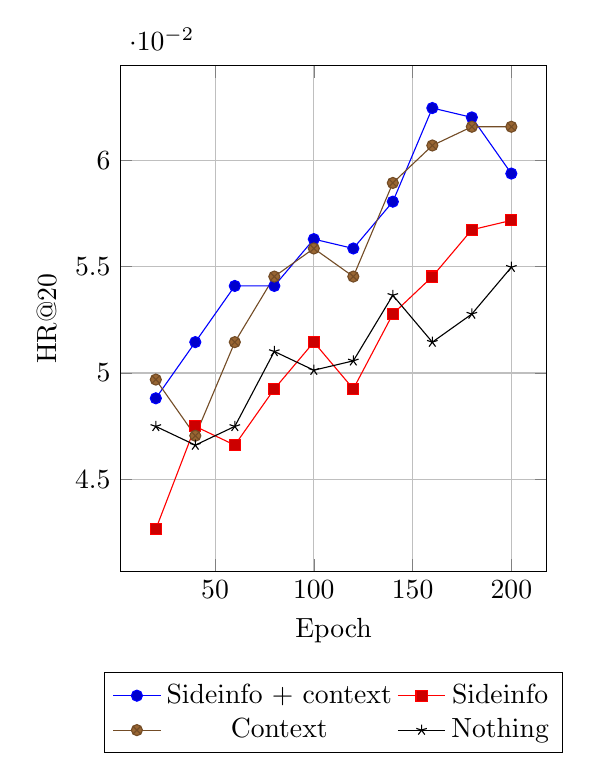
\begin{tikzpicture}
    \begin{axis}[
            xlabel=Epoch,
            ylabel=HR@20,
            height=8cm,
            width=7cm,
            grid=major,
            legend style={at={(0.5,-0.20)},
        anchor=north,legend columns=2}]
            
        \addplot plot coordinates{
            (20,0.04881)
            (40,0.05145)
            (60,0.05409)
            (80,0.05409)
            (100,0.05629)
            (120,0.05585)
            (140,0.05805)
            (160,0.06245)
            (180,0.06201)
            (200,0.05937)
        };

        \addplot plot coordinates {
            (20,0.04266)
            (40,0.04749)
            (60,0.04661)
            (80,0.04925)
            (100,0.05145)
            (120,0.04925)
            (140,0.05277)
            (160,0.05453)
            (180,0.05673)
            (200,0.05717)
        };

        \addplot plot coordinates {
            (20,0.04969)
            (40,0.04705)
            (60,0.05145)
            (80,0.05453)
            (100,0.05585)
            (120,0.05453)
            (140,0.05893)
            (160,0.06069)
            (180,0.06157)
            (200,0.06157)
        };

        \addplot plot coordinates {
            (20,0.04749)
            (40,0.04661)
            (60,0.04749)
            (80,0.05101)
            (100,0.05013)
            (120,0.05057)
            (140,0.05365)
            (160,0.05145)
            (180,0.05277)
            (200,0.05497)
        };
        \legend{Sideinfo + context,Sideinfo,Context,Nothing}
        \end{axis}
    \end{tikzpicture}
    \caption{The performance on HR@20 of CSGCN-IS on the Yelp-NC dataset with different types of input.}
    \label{subfig:ablation_study_context_specific_2}
    \end{subfigure}
    \caption{Ablation study for the input of CSGCN-ADJ and CSGCN-IS on Yelp-NC.}
\end{figure*}
\Cref{subfig:ablation_study_context_specific_1} shows the HR@20 for CSGCN-ADJ on Yelp-NC with different combinations of input. 
The results show that when side-information is included in the input for CSGCN-ADJ it does not change the performance much compared to excluding it.
Another interesting thing to note is how the model performs worse when context is included in the input, even though it is a context-specific setting.
This could be because the CSGCN-ADJ model does not actually model context in a way that fits the definition of context defined in \Cref{subsec:define_context_sideinfo}.
In CSGCN-ADJ, context can instead be viewed as a type of side-information, since it is modelled in a similar way.
Each user and item node is connected with the context value nodes of the contexts they have interacted in, just as they are connected to the nodes of their side-information values.
\\\\
\Cref{subfig:ablation_study_context_specific_2} shows HR@20 for CSGCN-IS on Yelp-NC with different inputs.
For CSGCN-IS, there is a slight increase in performance when side-information is included, compared to excluding it.
This shows that CSGCN-IS is able to use the side-information to better connect user and item nodes, increasing the collaborative signal.
We also see that for this model, including context in the input does make a significant different for the performance in a context-specific setting.
This is because context is modelled with finer granularity than in CSGCN-ADJ, meaning that each item and context value combination has an embedding.
The result of this finer granularity is that context can have different effects on the various items, resulting in more accurate context-specific recommendations.
In general, side-information can have a slight effect on the results depending on the type of model.
However, the context seems to have a lot larger effect on the performance of the models, as would be expected for context-aware recommendation.
Additionally, it may be worth noting that the context used for these experiments is mainly based on discretized values based on timestamps, which might not be a useful contextual dimension due to timezone differences.
We do not see any overwhelming evidence that side-information is able to improve context-aware recommendations.
